\documentclass[letterpaper]{article} % Feel free to change this
\usepackage[margin=1in]{geometry}
\usepackage{float}
\usepackage{graphicx}
\usepackage{listings}

\begin{document}

\title{ECE 350: Digital Systems Final Project}
\author{Daniel Winkelman} % Change this to your name
\date{\today} % Change this to the date you are submitting
\maketitle
\noindent
All source code is available at \texttt{https://github.com/dwinkelman0/ECE350Final}. The assembly code used to test this project is too extensive to include entirely in this report.

\section*{Duke Community Standard}
I affirm that each submission complies with the Duke Community Standard and the guidelines set forth for this assignment.

\section{Introduction}
It is essential that digital systems have the ability to communicate information from a source to a destination. However, all transmission media are "noisy", having the potential to introduce errors in which the received signal differs from the original. This is problematic because many applications of digital communication are vulnerable to small corruptions arising from flipped bits. Hamming coding mitigates the effects of noisy channel errors by incorporating redundant data into the transmitted signal, enabling a vast majority of errors to be corrected or detected.\\

\begin{figure}
\begin{center}
	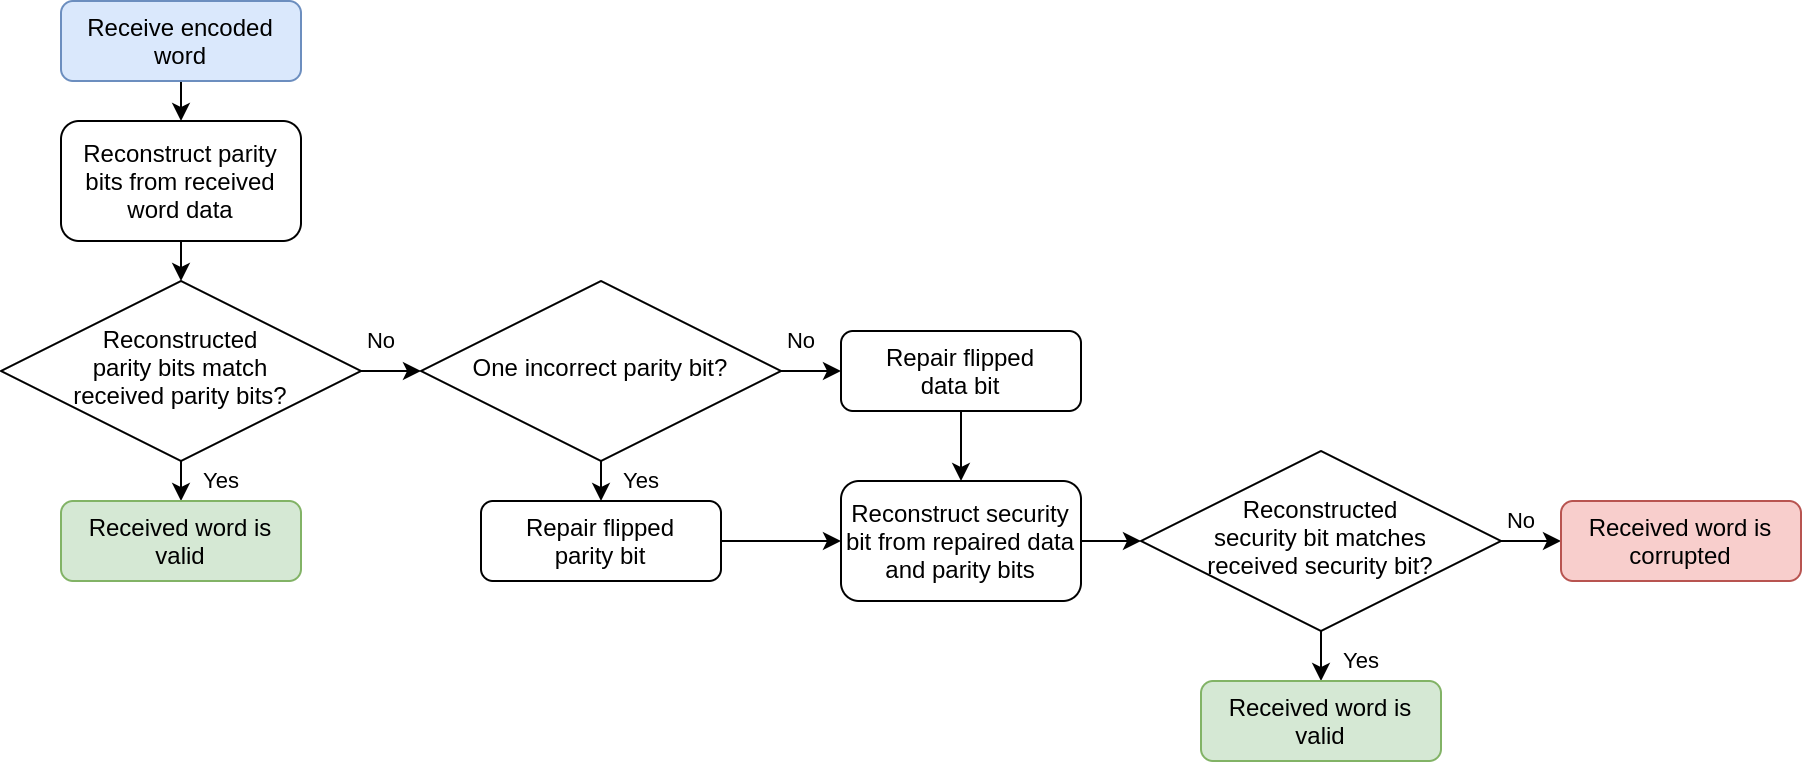
\includegraphics[width=1\textwidth]{decoding.png}
	\caption{The decoding algorithm for a SECDED Hamming code.}
	\label{fig:decoding_algorithm}
\end{center}
\end{figure}

\noindent
Hamming(31,26) coding is one particular configuration of the Hamming coding technique. Encoded words cover 26 bits of data and contain 5 parity bits; an additional security bit is the even parity of the 31 data and parity bits. This code is SECDED (single error correcting, double error detecting). It is assumed that no more than two bits are flipped during transmission; the algorithm is not guaranteed to detect or correct errors if more than two bits are flipped. Figure \ref{fig:decoding_algorithm} illustrates the decoding algorithm.\\

\noindent
This project explores the implementation of Hamming(31,26) coding on a hardware level. The objectives of this project include:
\begin{enumerate}
	\item implement instructions for Hamming(31,26) encoding and decoding in the MIPS-like Logisim processor developed in Project Checkpoint 4
	\item implement of instructions in the assembler
	\item write a MIPS program to thoroughly test instructions
	\item write a MIPS program to simulate an application of the instructions in the context of a noisy channel
\end{enumerate}

\section{Instructions}
Figure \ref{fig:instructions} lists the instructions implemented in the processor as part of this project. Figure \ref{fig:encoder_circuit} shows the circuit implementing the encoder and Figure \ref{fig:decoder_circuit} shows the circuit implementing the decoder. The additional instructions (particularly XOR) were added to facilitate the testing programs.
\begin{center}
\begin{figure}
	\begin{tabular}{|l|c|c|p{7cm}|}
		\hline
	Instruction & Opcode & ALU Op & Description \\ \hline
		\texttt{henc \$rd, \$rs} & 00000 & 00110 & Encode the 26 LSB's in \texttt{\$rs} to a 32-bit Hamming word in \texttt{\$rd} \\ \hline
		\texttt{hdec \$rd, \$rs} & 00000 & 00111 & Decode the Hamming word in \texttt{\$rs} to a 26-bit word in \texttt{\$rd}; if double error detected, writes \texttt{0x4} into \texttt{\$rstatus} and does not change \texttt{\$rd} \\ \hline
		\texttt{xor \$rd, \$rs, \$rt} & 00000 & 01000 & Bitwise XOR operation on two words \\ \hline
		\texttt{not \$rd, \$rs} & 00000 & 01001 & Bitwise NOT operation \\ \hline
		\texttt{pcnt \$rd, \$rs} & 00000 & 01010 & Count the number of bits in \texttt{\$rs} set to 1 \\ \hline
	\end{tabular}
	\caption{Instructions implemented in the processor.}
	\label{fig:instructions}
\end{figure}
\end{center}
\begin{center}
\begin{figure}
	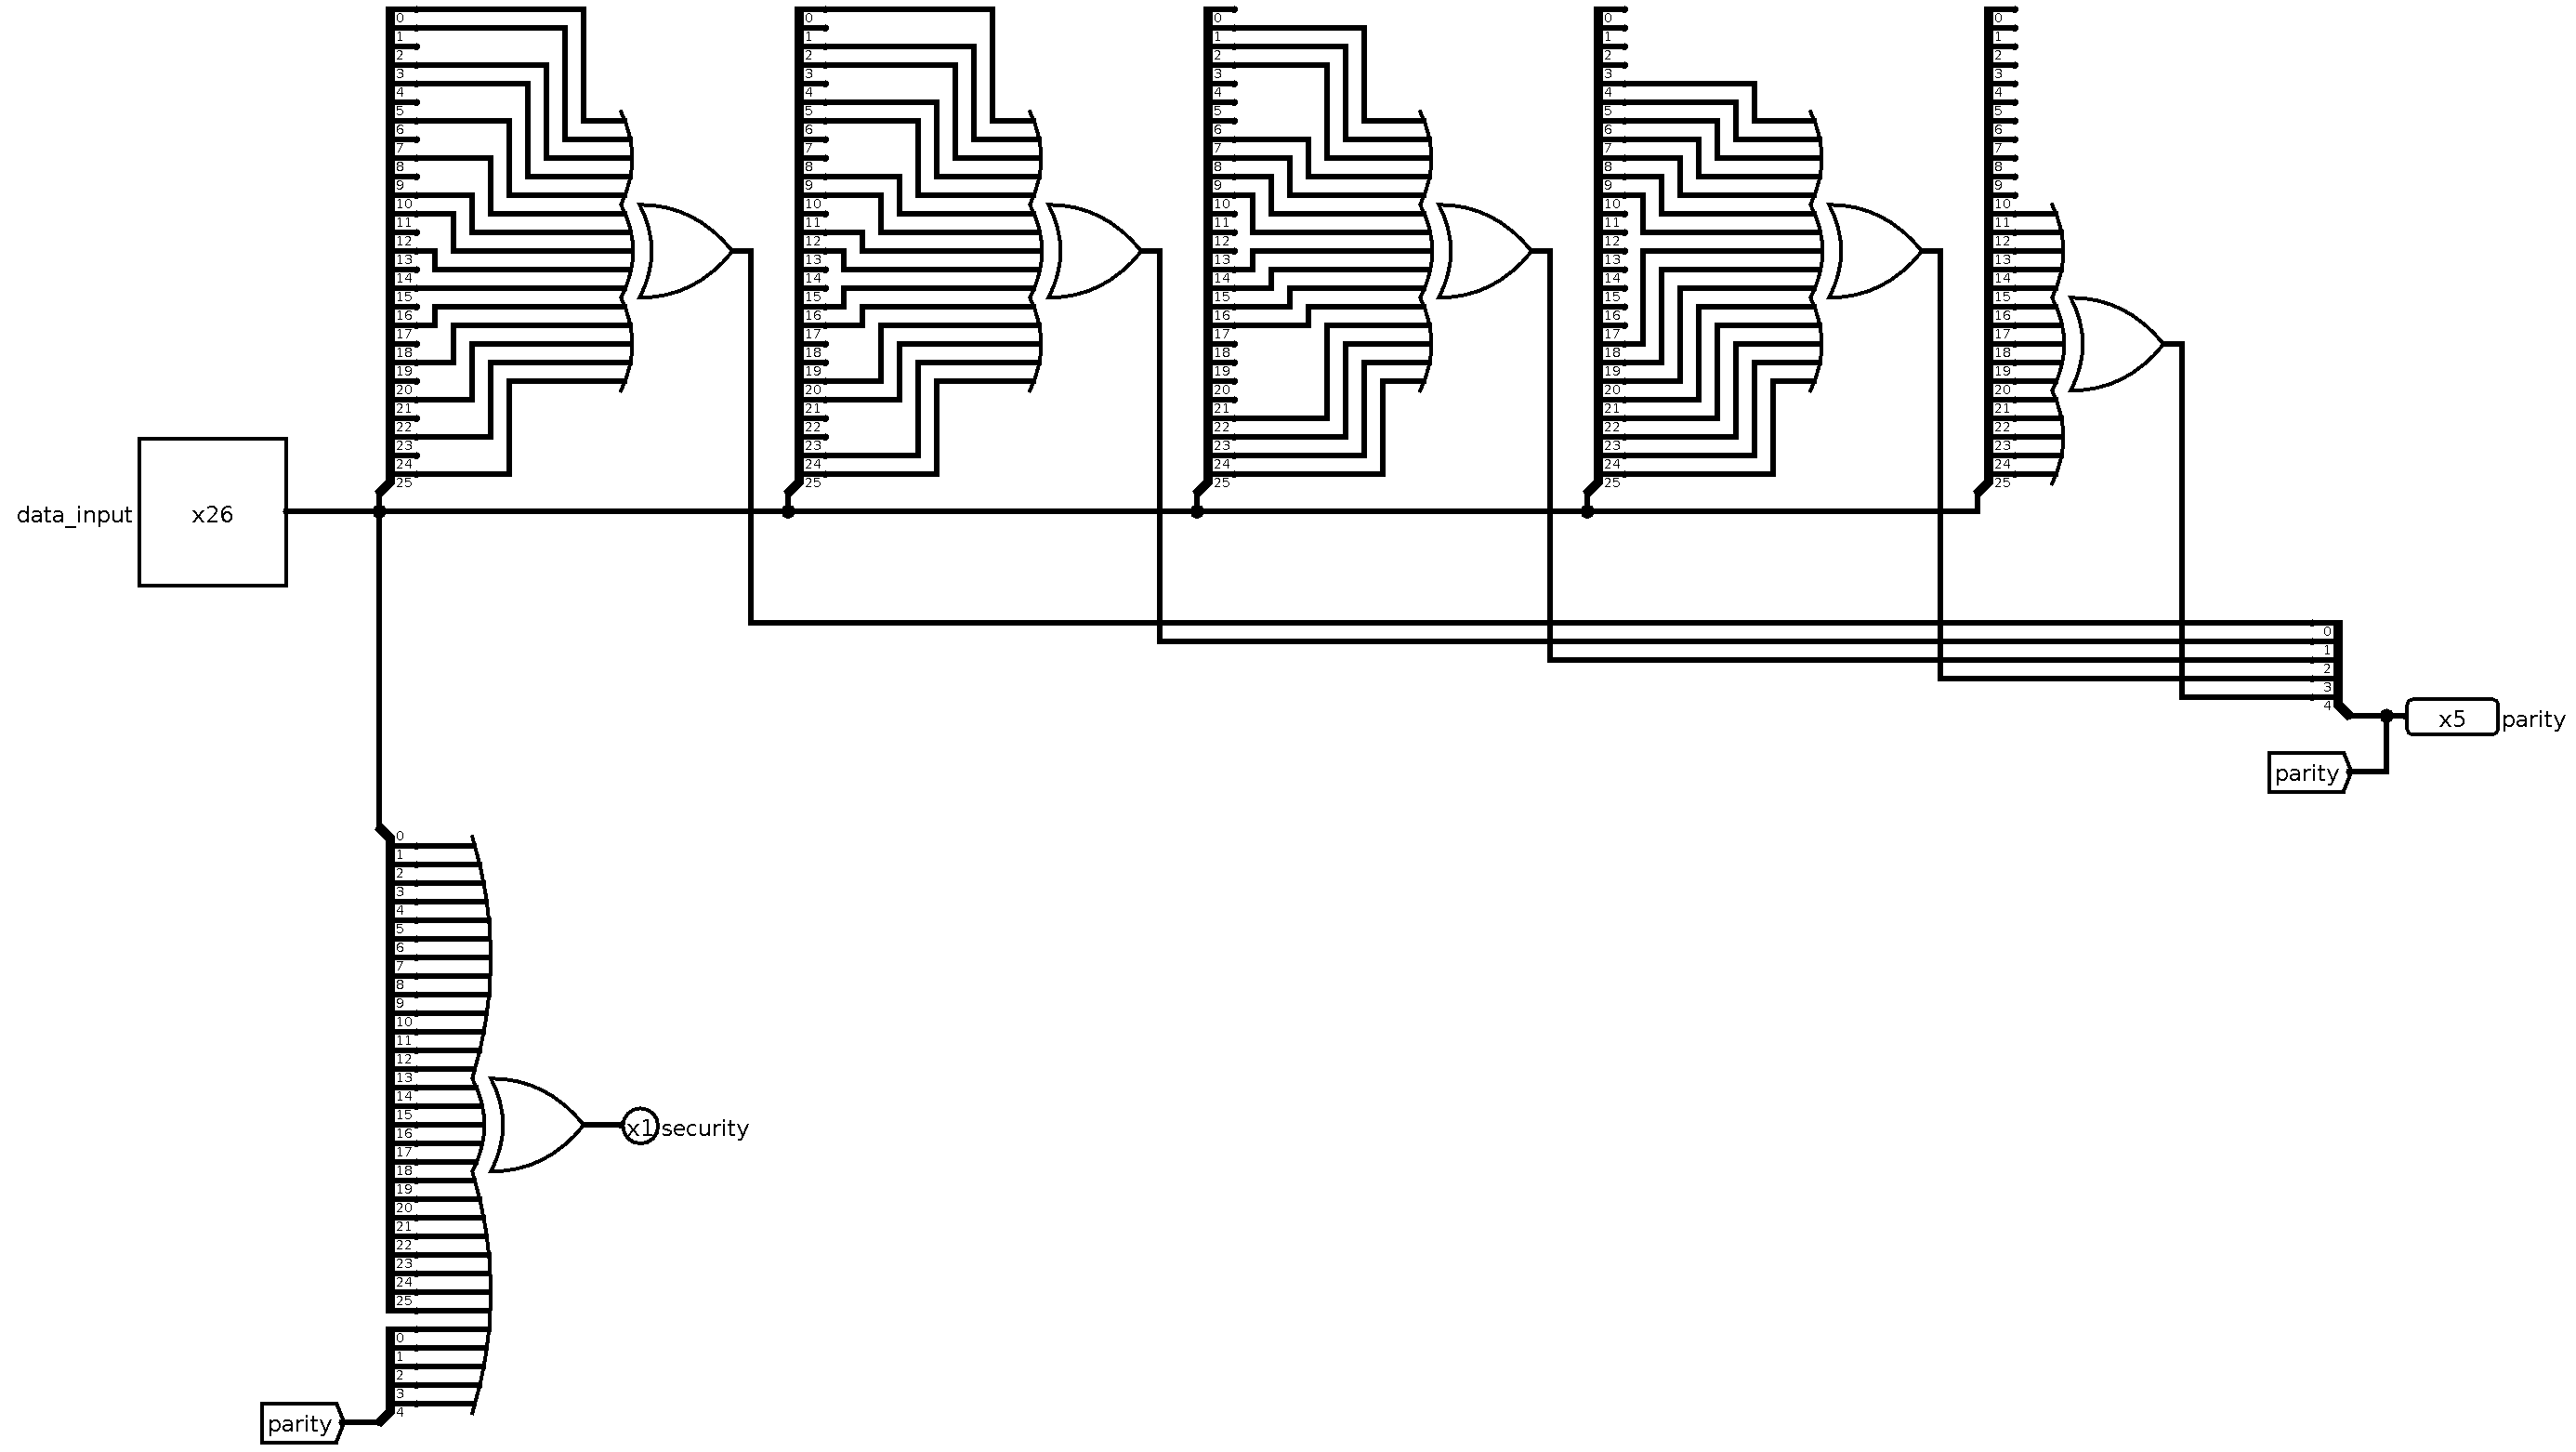
\includegraphics[width=1\textwidth]{encoder_circuit.png}
	\caption{Circuit implementing the encoder instruction.}
	\label{fig:encoder_circuit}
\end{figure}
\end{center}
\begin{center}
\begin{figure}
	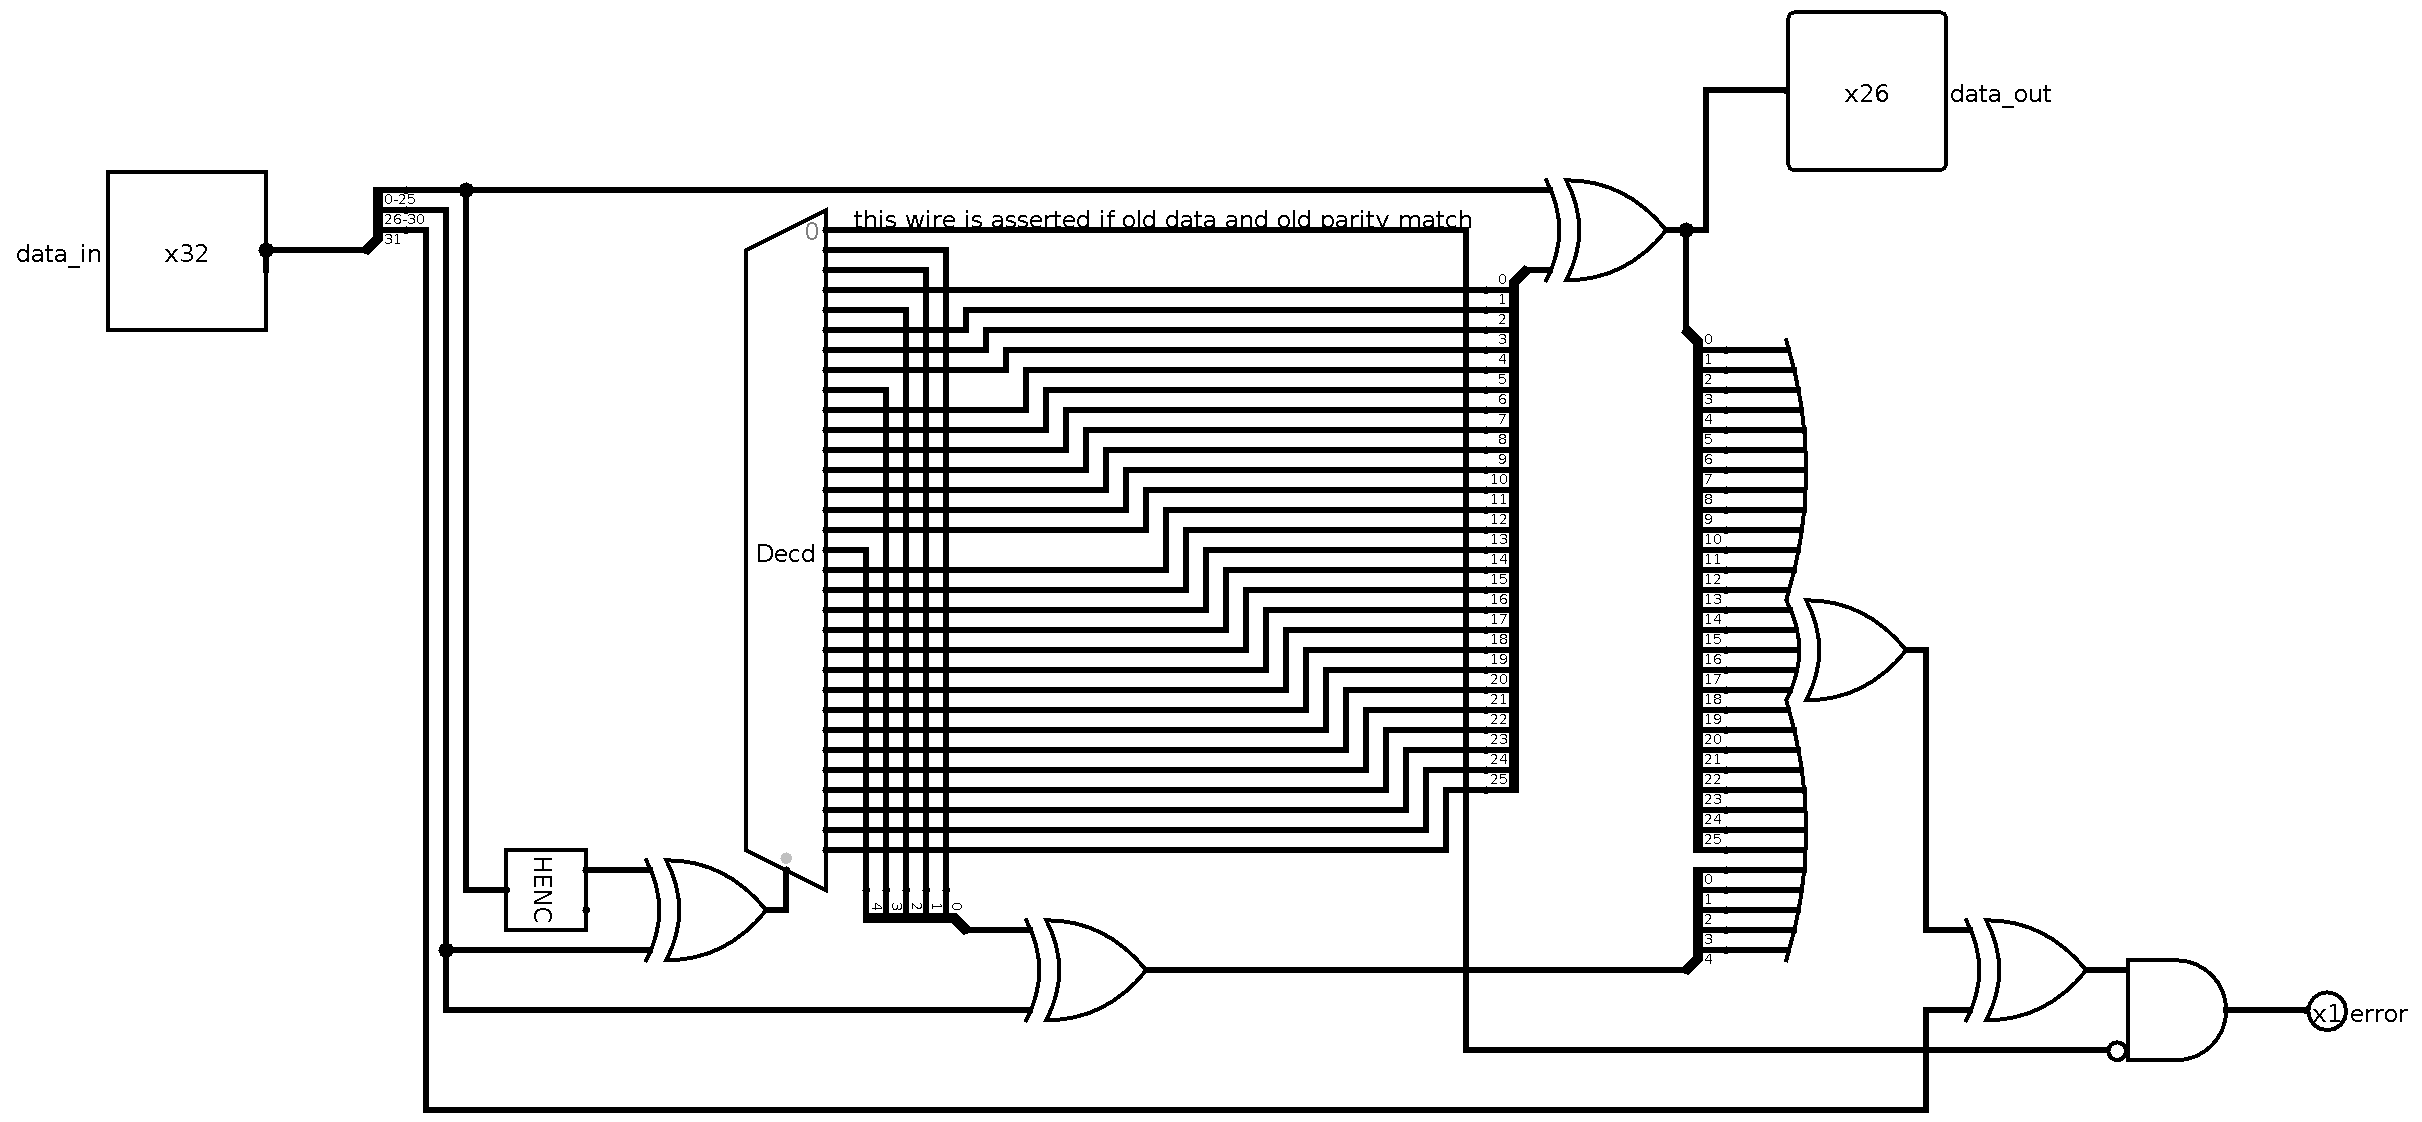
\includegraphics[width=1\textwidth]{decoder_circuit.png}
	\caption{Circuit implementing the decoder instruction. This circuit directly implements the algorithm illustrated in Figure \ref{fig:decoding_algorithm}. The decoder element in the circuit uses the difference between the computed parity bits from the received data and the received parity bits to determine which bit was flipped if it is assumed that only one bit was flipped.}
	\label{fig:decoder_circuit}
\end{figure}
\end{center}

\section{Instruction Testing}
Assembly scripts were used to nearly-exhaustively test the encoding and decoding instructions. An Xorshift shift-register generator was implemented to generate random 26-bit words; a random word is encoded using the \texttt{henc} instruction, noise is applied to the Hamming word using an \texttt{xor} operation, and the Hamming word is decoded using the \texttt{hdec} instruction. If no noise or one bit of noise is applied, the original word is expected; if two bits of noise is applied, non-zero \texttt{\$rstatus} is expected.\\

\noindent
Six classes of test cases were identified. Of these, it was practical to exhaustively four classes; the remaining classes were tested with a large number of cases.
\begin{itemize}
	\item No noise (exhaustive)
	\item 1 bit is flipped (exhaustive)
	\item 2 data bits are flipped
	\item 2 parity bits are flipped (exhaustive)
	\item 1 data bit and 1 parity bit are flipped
	\item Security bit and 1 other bit are flipped (exhaustive)
\end{itemize}

\noindent
The following, which tests the case in which two parity bits are flipped, is representative of all six classes:
\begin{lstlisting}
test_sequence_2n_pp:
	addi $r11, $r0, 4
	sll  $r11, $r11, 28
	addi $r13, $r0, 8
	addi $r14, $r0, 16
	addi $r31, $r0, test_sequence_2n_pp_loop_return_point
	
test_sequence_2n_pp_loop:
	add  $r12, $r13, $r14
	or   $r7, $r11, $r12
	sll  $r12, $r12, 26
	henc $r8, $r4
	xor  $r8, $r8, $r12
	hdec $r9, $r8
	j    test_sequence_check_success

test_sequence_2n_pp_loop_return_point:
	sra  $r13, $r13, 1
	bne  $r13, $r0, test_sequence_2n_pp_loop
	sra  $r14, $r14, 1
	sra  $r13, $r14, 1
	bne  $r13, $r0, test_sequence_2n_pp_loop
\end{lstlisting}

\section{Demo Program}
A brief program was written to demonstrate how the instructions would be used in a more realistic setting. A sequence of squares is generated to serve as the message to transmit. After each message of the word is encoded, a sparse noise word is generated by AND-ing together five random words (meaning that each bit in the noise word has a $\frac{1}{32}$ chance of being 1). A Poisson distribution can be used to estimate the probability that a noise word contains a total number of noise bits. Once all words have been encoded and had noise applied, all words are decoded; if a double error is detected, the decoding loop requests that the corrupted word be resent. Since there is no guarantee that noise words have two or fewer noise bits, some corrupted data will appear after decoding.

\section{Conclusions}
\subsection{Challenges}
The greatest challenge in completing this project was reasoning about efficient ways to detect and correct single and double errors. In class, the emphasis was placed on encoding, but the decoding algorithm was never fleshed out in great detail.\\

\noindent
Ensuring the quality of the testing programs was also challenging. Planning the structure of the program in advance was important because the different classes of tests had considerable commonality, but each test class still required perfect assembly code. Once the first batch of tests was devised in a scalable way, it was easier to implement the rest of the tests.

\subsection{Further Work}
There are a couple natural extensions to the work done in this project:
\begin{itemize}
	\item \textbf{Implement Hamming(63,57).} Hamming(63,57) coding has less overhead than Hamming(31,26) but less capacity per bit to detect errors, making it better-suited to communications channels with relatively low amounts of noise. In this processor, encoding and decoding instructions could be implemented in two halves that accept the high and low portions of words in two parameters and produce outputs in two halves. Using internal specialized registers could help scale this technique to higher word sizes.
	\item \textbf{Direct memory access.} The implemented instructions face a key limitation in the number of supporting operations which must take place around encoding and decoding instructions, like memory access and loop management. A more dynamic approach would integrate instructions which interact with the memory directly to avoid this overhead. However, this adds a large degree of complexity to the pipelined state machine model the processor is based upon. Such a system would require additional infrastructure like specialized internal registers and new approaches to exception handling. Building a co-processor with direct memory access, similar to modern WiFi chips, would be a more scalable approach.
\end{itemize}

\end{document}
